\chapter{Experiments}

The aim of experiments is a validation of system's functionality. According to plan, the system was firstly calibrated and tuned. Sensors' calibration was conducted on a flat surface, before mounting. Next fusion's parameters were tuned when sensor mounted on moves along previously prepared trajectories.\\

 First, the orientation estimation was examined. The node was rigidly linked to the robot's tip. A figure (\ref{sensor_mount}) presents sensor mounted in the robot's gripper. The sponges were used to mitigate vibrations.  Then, the robot executed a predetermined motion in which the position remained constant while only the orientation changed, among five learned configurations. The orientation calculated by the robot's control system was compared with the orientation estimated by the inertial sensors. Due to lack of magnetometer the yaw angle could not be properly estimated so its analyzes was skipped. However, the yaw angle can be fixed by using appropriate constraint (equation \ref{yaw_constraint_fun}). The experiment was repeated without and with constraint's correction and with various speeds. A listing (\ref{karel1}) presents the KAREL program that realizes this trajectory.
 
 \begin{lstlisting}[caption={The KAREL program realizing an orientation changes}, captionpos=b, label=karel1]
 	To fill up...
 \end{lstlisting}
 
\begin{figure}[!h]
	\centering
	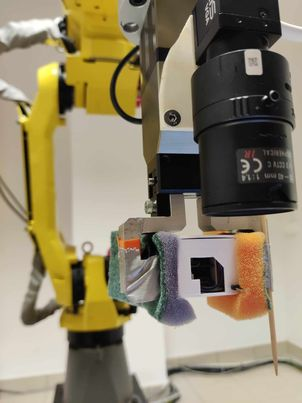
\includegraphics[width=0.6\textwidth]{sensor_mount.jpg}
	\caption{Sensor mounted in the robot's gripper}
	\label{sensor_mount}
\end{figure}

 Next, the system was examined under the default operating conditions -- estimates the position and the orientation. The node was mounted on plate that starts circular movement with different frequency and direction, according to mechanism constraints. The estimation was conducted in multiple configuration, that included:
\begin{itemize}
	\item case A -- position provider + gyroscope (accelerometer was used only to correct orientation),
	\item case B -- position provider + gyroscope + accelerometer + constraint's correction,
	\item case C -- position provider + constraint's correction,
	\item case D -- position provider + gyroscope + accelerometer,
	\item case E -- position provider + gyroscope + accelerometer + constraint's correction
	\item case F -- position provider + gyroscope + accelerometer + simplified constraint's correction
\end{itemize}

The configuration without position provider was also examined, but the results obtained were much worse in terms of quality. During experiments it is assumed that orientation does not change and the position provided sample rate was limited to 2 Hz. The trajectory generated by the industrial robot is similar to that given in the equations (\ref{tcp_begin} - \ref{tcp_end}), but due to the robot's control system limitation the speed is discreetly increased twice per revolution. A listing (\ref{karel2}) presents the KAREL program that realizes this trajectory.

\begin{lstlisting}[caption={The KAREL program realizing a circular motion}, captionpos=b, label=karel2]
	To fill up...
\end{lstlisting}

\section{Results}

The gathered logs were post-processed and compared using MATLAB scripts. Figures (\ref{ori_est_roll} - (\ref{ori_est_yaw})) present the orientation's estimation from the first experiment. The estimated orientation angles are compared with the orientation calculated by the robot's positioning system.\\

Figures (\ref{pos_est_x} - (\ref{ori_est_yaw2}) present the position and orientation estimations obtained for the proposed configuration. It is expected that x and y coordinates estimate circular motion, while the z and orientation angles remain zeros.\\

The profit from an application of the constraints' correction is eminently visible when corrections with various "strength" are compared.
A figure (\ref{corr_strength}) presents an estimation of position in circular motion for different parameters (see equation (\ref{constraint_final})). The sample rate of external position provider is constant, so there is increasingly less update for every rotation. If correction is not active, the estimation tends to drift in the peaks. However, the "stronger" correction is active, the less error in those moments.


\begin{figure}[p]
	\centering
	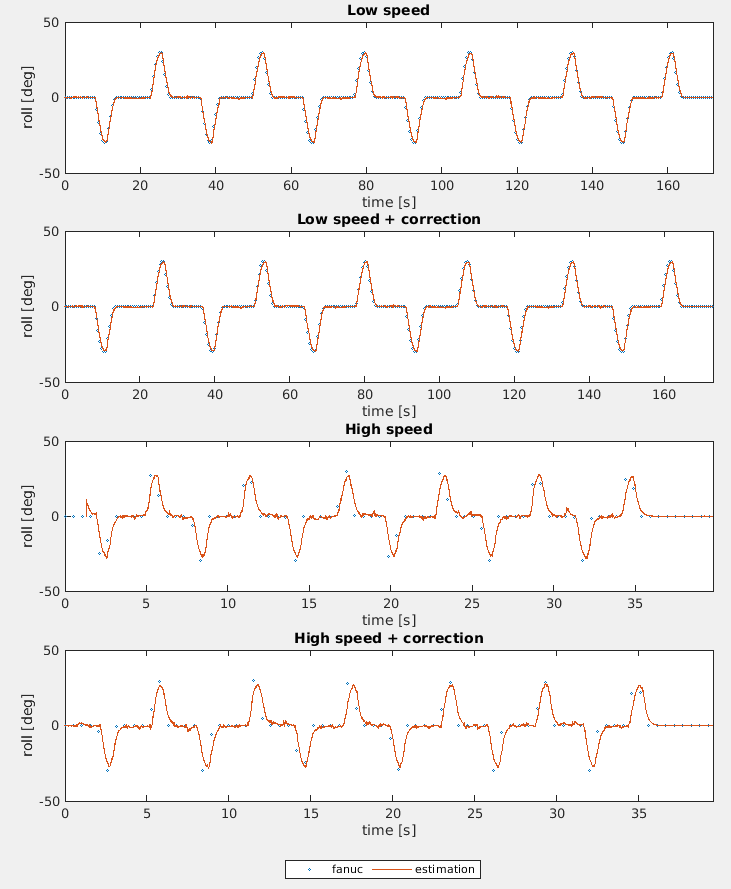
\includegraphics[width=\textwidth]{ori_est_roll.png}
	\caption{Experiment 1: orientation estimation -- roll}
	\label{ori_est_roll}
\end{figure}

\begin{figure}[p]
	\centering
	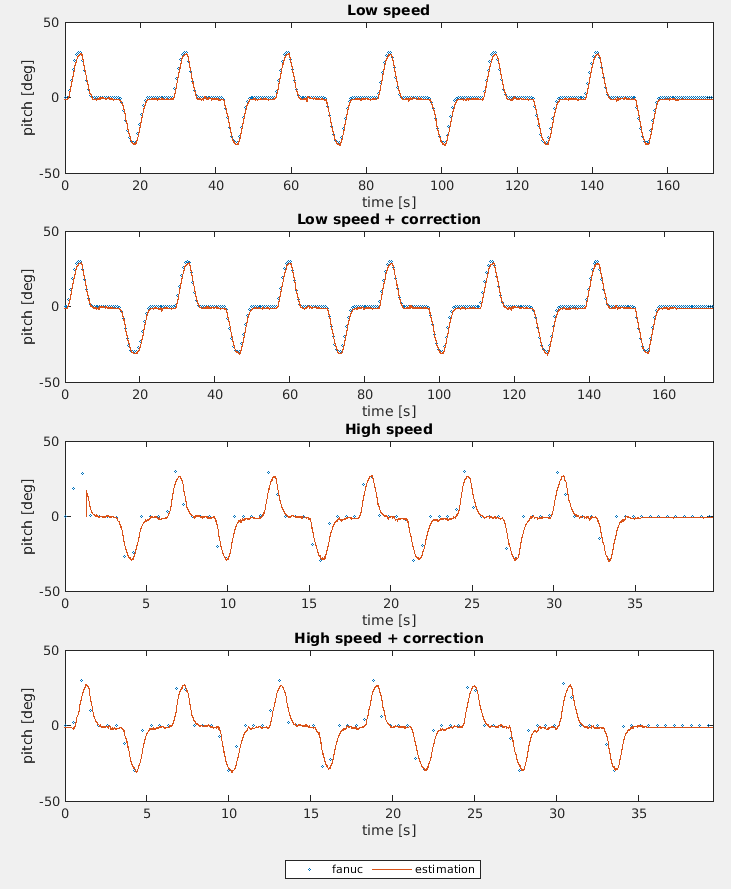
\includegraphics[width=\textwidth]{ori_est_pitch.png}
	\caption{Experiment 1: orientation estimation -- pitch}
	\label{ori_est_pitch}
\end{figure}


\begin{figure}[p]
	\centering
	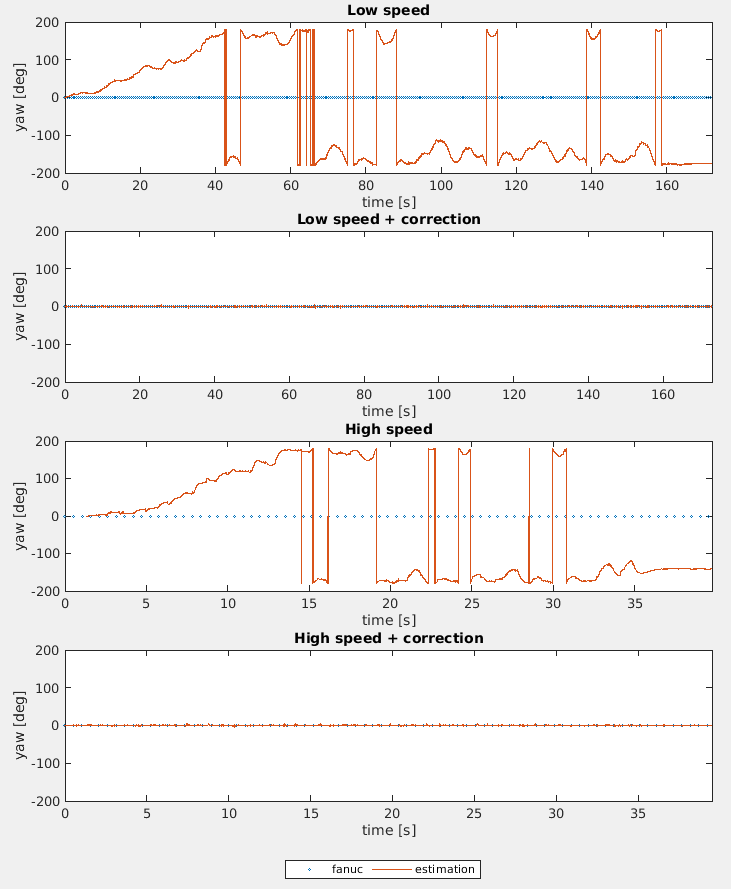
\includegraphics[width=\textwidth]{ori_est_yaw.png}
	\caption{Experiment 1: orientation estimation -- yaw}
	\label{ori_est_yaw}
\end{figure}

\begin{figure}[p]
	\centering
	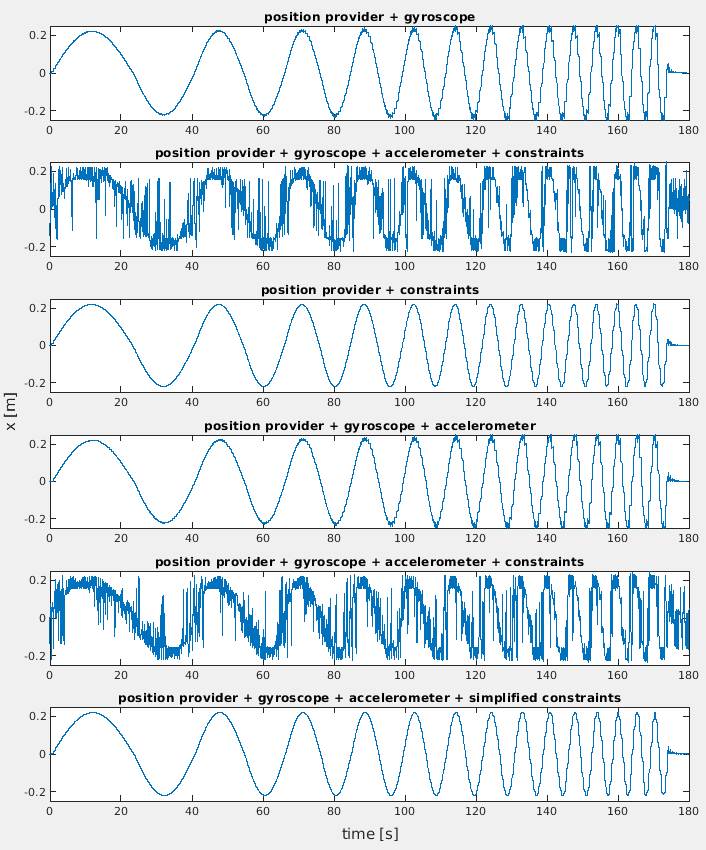
\includegraphics[width=\textwidth]{pos_est_x.png}
	\caption{Experiment 2: position estimation -- x}
	\label{pos_est_x}
\end{figure}

\begin{figure}[p]
	\centering
	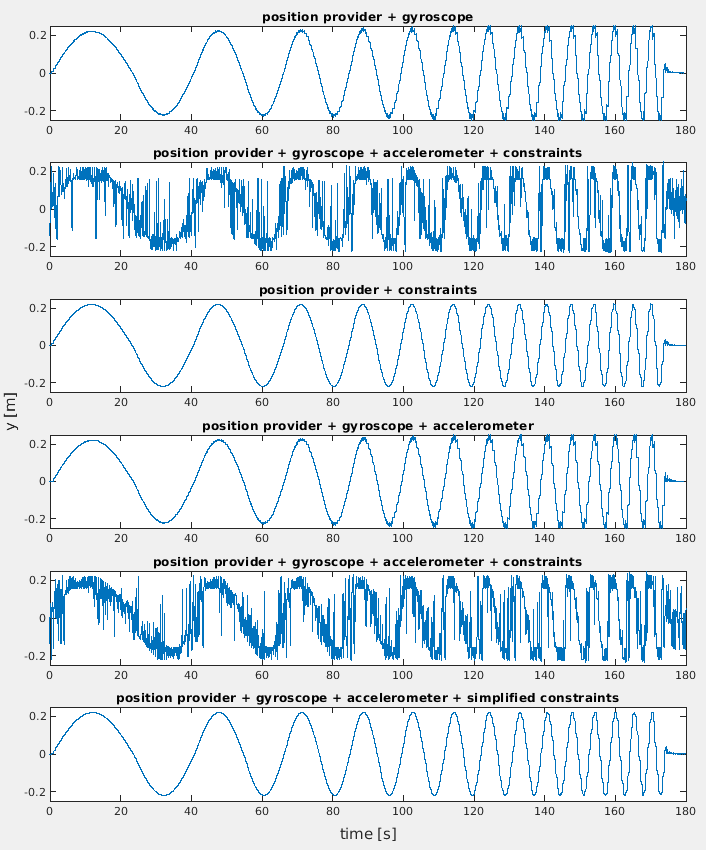
\includegraphics[width=\textwidth]{pos_est_y.png}
	\caption{Experiment 2: position estimation -- y}
	\label{pos_est_y}
\end{figure}

\begin{figure}[p]
	\centering
	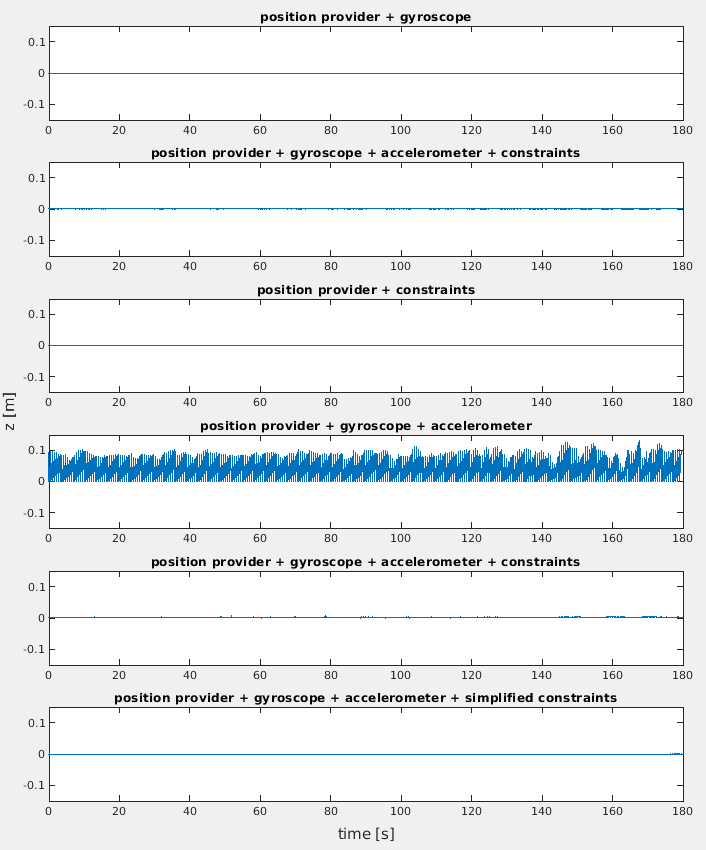
\includegraphics[width=\textwidth]{pos_est_z.png}
	\caption{Experiment 2: position estimation -- z}
	\label{pos_est_z}
\end{figure}

\begin{figure}[p]
	\centering
	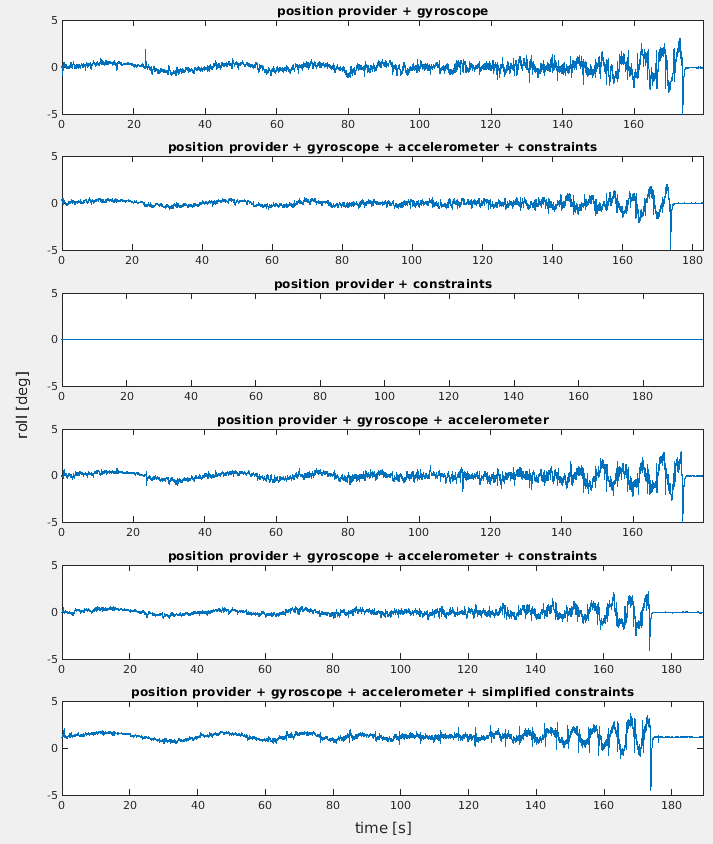
\includegraphics[width=\textwidth]{ori_est_roll2.png}
	\caption{Experiment 2: orientation estimation -- roll}
	\label{ori_est_roll2}
\end{figure}

\begin{figure}[p]
	\centering
	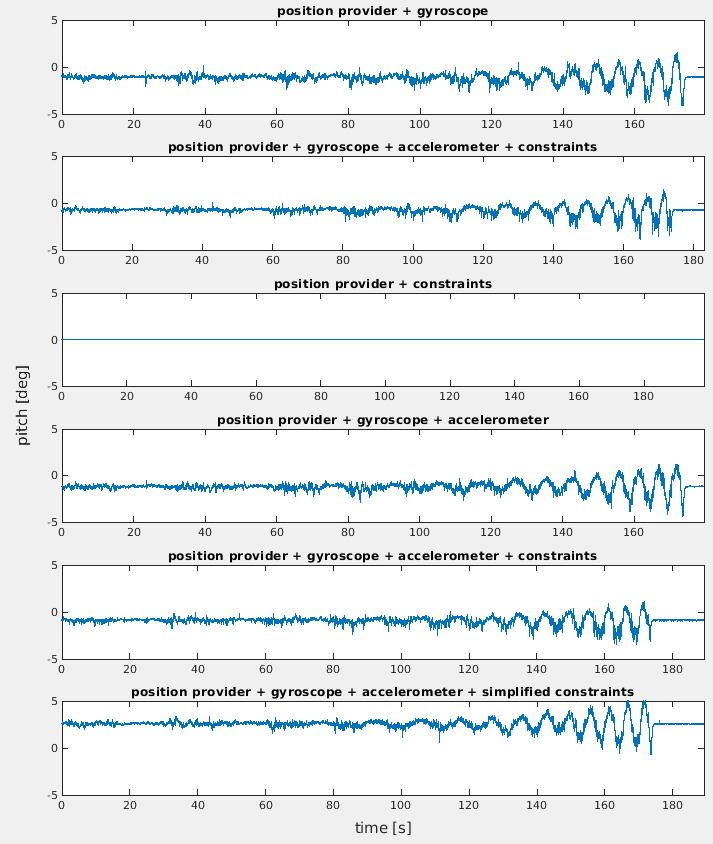
\includegraphics[width=\textwidth]{ori_est_pitch2.png}
	\caption{Experiment 2: orientation estimation -- pitch}
	\label{ori_est_pitch2}
\end{figure}


\begin{figure}[p]
	\centering
	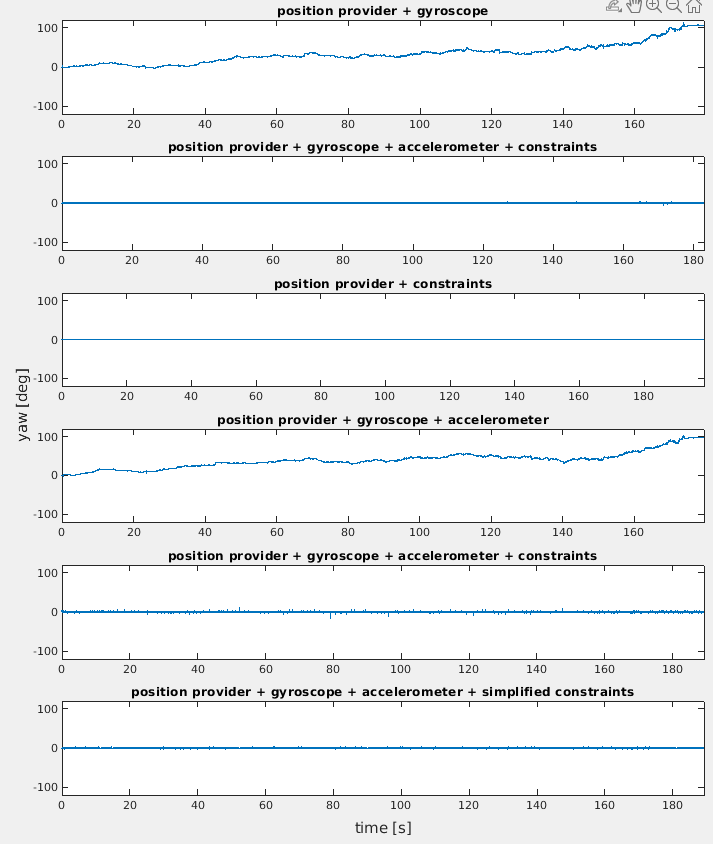
\includegraphics[width=\textwidth]{ori_est_yaw2.png}
	\caption{Experiment 2: orientation estimation -- yaw}
	\label{ori_est_yaw2}
\end{figure}


\begin{figure}[p]
	\centering
	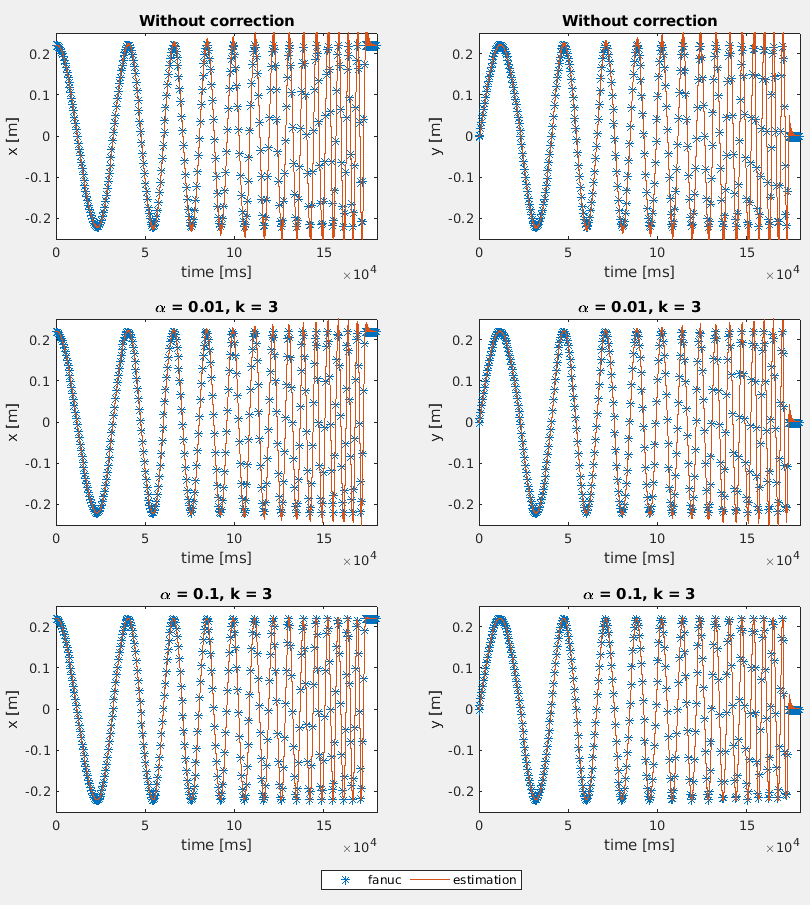
\includegraphics[width=\textwidth]{corr_influence.png}
	\caption{Tuning: the influence of constraints' correction}
	\label{corr_strength}
\end{figure}

